\documentclass{svproc}
%
% RECOMMENDED %%%%%%%%%%%%%%%%%%%%%%%%%%%%%%%%%%%%%%%%%%%%%%%%%%%
%

\usepackage{amssymb}
%% The amsmath package provides various useful equation environments.
\usepackage{amsmath}
%% The amsthm package provides extended theorem environments
% \usepackage{amsthm}

% Pseudocode
\usepackage{algorithm}
\usepackage{algorithmic}

\usepackage{booktabs}

%% The lineno packages adds line numbers. Start line numbering with
%% \begin{linenumbers}, end it with \end{linenumbers}. Or switch it on
%% for the whole article with \linenumbers.
%% \usepackage{lineno}

\usepackage{array}

% to typeset URLs, URIs, and DOIs
\usepackage{url}
\def\UrlFont{\rmfamily}

\begin{document}
\mainmatter              % start of a contribution
%
\title{T-NOTE: Transformer Encoder for Task Offloading in Edge-Fog-Cloud Computing Environments}
%
\titlerunning{T-NOTE}  % abbreviated title (for running head)
%                                     also used for the TOC unless
%                                     \toctitle is used
%
\author{Arthur Garon\inst{1} \and Sonia Yassa\inst{2}
Lylia Alouache\inst{3}}
%
\authorrunning{Arthur Garon et al.} % abbreviated author list (for running head)
%
%%%% list of authors for the TOC (use if author list has to be modified)
\tocauthor{Arthur Garon, Sonia Yassa, Lylia Alouache}
%
\institute{CY Cergy Paris Université,\\
\email{I.Ekeland@princeton.edu},\\ WWW home page:
\texttt{http://users/\homedir iekeland/web/welcome.html}
\and
Universit\'{e} de Paris-Sud,
Laboratoire d'Analyse Num\'{e}rique, B\^{a}timent 425,\\
F-91405 Orsay Cedex, France}

\maketitle              % typeset the title of the contribution

\begin{abstract}
The abstract should summarize the contents of the paper
using at least 70 and at most 150 words. It will be set in 9-point
font size and be inset 1.0 cm from the right and left margins.
There will be two blank lines before and after the Abstract. \dots
% We would like to encourage you to list your keywords within
% the abstract section using the \keywords{...} command.
\keywords{computational geometry, graph theory, Hamilton cycles}
\end{abstract}
%


\section{Introduction}\label{sec:introduction}

\subsection{Background and motivation}\label{subsec:background}


The Internet of Things (IoT) has become a foundational element of modern technology, facilitating the development of innovative applications in domains such as smart cities, healthcare, autonomous systems, and other fields. The proliferation of IoT devices has been rapid and significant, with Cisco reporting a global total exceeding 30 billion~\cite{benaboura_comprehensive_nodate}. These devices generate a substantial volume of data, approximately 2 exabytes on a daily basis. Achieving maximum potential from these systems necessitates the implementation of efficient processing and analysis methodologies. This requirement presents a formidable challenge in the domains of data management, resource allocation, and system scalability.

The inherent limitations of IoT devices, such as their small batteries, limited processing power, and minimal storage capacity, render them ill-suited to manage the substantial volumes of data they generate. Tasks such as real-time processing of sensor data or computation-intensive applications frequently exceed the capabilities of local devices. Conventional approaches entail the delegation of these tasks to centralized cloud servers. However, network limitations and latency sensitivity frequently render this approach inefficient, particularly for real-time applications~\cite{benaboura_comprehensive_nodate}.

To address these challenges, fog computing has emerged as a distributed computing paradigm that extends the capabilities of cloud computing to the edge of the network. By facilitating the execution of storage, computation, and data management operations in close proximity to the data source, fog computing contributes to the reduction of latency, power consumption, and network traffic. It is evident that contemporary applications, including but not limited to smart homes, autonomous vehicles, smart agriculture, and healthcare, are contingent on this paradigm to satisfy their real-time and location-aware processing requirements as evoked by~\cite{das_review_2023}. Fog computing, first introduced in 2012, provides a hierarchical architecture that serves to bridge the gap between cloud servers and IoT devices, thereby allowing for seamless data flow and operational efficiency~\cite{fahimullah_review_2022}.

Despite the advantages inherent in task offloading in fog computing, this process is encumbered by numerous challenges. Optimizing resource utilization, reducing energy consumption, and maintaining Quality of Service (QoS) require robust strategies due to the heterogeneous and dynamic nature of fog networks. Factors such as fluctuating workloads, mobility, and task diversity have been identified as contributing to an increase in the complexity of the situation. To address these challenges, innovative resource allocation techniques are required, including Machine Learning-based (ML) methods, auction models, and heuristic optimization as~\cite{fahimullah_review_2022} exhibits.

Conventional resource management techniques frequently employ static heuristic approaches, which prove ineffective when confronted with the diverse and dynamic workloads that are characteristic of fog environments. They exhibit a deficiency in scalability and flexibility, which are prerequisites for real-time task offloading and resource optimization. Consequently, a substantial decline in performance is experienced as system demands increase~\cite{iftikhar_ai-based_2023}.

To address this problem, metaheuristics such as GA have emerged in the field of offloading as powerful optimization techniques capable of handling the multi-objective nature of fog computing task offloading. GAs excel in exploring complex solution spaces and finding near-optimal trade-offs between conflicting objectives such as latency minimization, energy efficiency, and resource utilization. Unlike traditional optimization methods that often focus on single objectives, multi-objective genetic algorithms can simultaneously optimize multiple performance criteria, making them particularly suitable for fog computing environments where various QoS parameters must be balanced. The evolutionary nature of GAs allows them to adapt to dynamic network conditions and heterogeneous resource availability, providing robust solutions for real-time task offloading decisions.

Recent advancements in the field of Artificial Intelligence (AI), particularly deep reinforcement learning (DRL), have demonstrated considerable potential in addressing the intricacies of task offloading in fog environments. Research has demonstrated the efficacy of AI-driven approaches in reducing latency, energy consumption, and operational costs. As~\cite{fahimullah_review_2022} demonstrates in their review, techniques such as centralized Dueling Deep Q-Networks (DDQNs), decentralized learning models, and multi-agent reinforcement learning have been employed to optimize offloading policies and resource allocation. Furthermore, hybrid strategies that integrate artificial intelligence with conventional methods have demonstrated efficacy in heterogeneous fog environments~\cite{mishra_collaborative_2023}.

In order to maintain currency with the latest advancements in this domain, the present study investigates innovative methodologies that integrate the strengths of evolutionary computation and deep reinforcement learning for the purpose of optimizing IoT task offloading. The integration of these approaches addresses the limitations of individual techniques while leveraging their complementary advantages.


\subsection{Contributions}

To address these gaps, this work makes the following key contributions:
\begin{itemize} 
    \item The proposal of two transformer-based architectures, utilizing DQL for the purpose of task offloading within a cloud-fog-edge environment. The selection of the node (edge, fog or cloud) to execute each incoming task is determined by these models, representing n different actions. The NOTE system is oriented towards node-level features, such as CPU, buffer, and bandwidth. In contrast, the T-NOTE system incorporates additional task attributes, including size, deadline, and CPU-cycle requirements. This capability facilitates a more precise depiction of the interplay between node resources and task demands within a fog environment.

    \item This work also puts forth a model for offloading in hybrid environments that considers a substantial number of parameters for the QoS. To further expand upon the existing body of knowledge, we implement an adaptation of a scenario with a real dataset within the framework of RayClousSim. We make the scenario and the dataset open-source for the community\footnote{\url{https://github.com/tutur90/Task-Offloading-Fog}}. All algorithms used, including NOTE and T-NOTE, are also implemented in this framework.

    \item Additionally, we conduct a comparative analysis between GAs and a DQL approach. The implementation of these algorithms in the training of an MLP constitutes a pivotal element of the study. The GA approach is employed in a dynamic setting, thereby enabling the MLP to be optimized for multi-objective offloading in real time.
\end{itemize}


\subsection{Paper organization}

The reminder of this paper is structured as follows: Section~\ref{sec:related_work} reviews related work; Section~\ref{sec:problem_modeling} describes the problem modeling, including the scenario and QoS modeling; Section~\ref{sec:offloading_strategies} details the proposed strategies, from genetics algorithm to deep reinforcement learning approaches, including Transformers-based methods; Section~\ref{sec:performance_evaluation} presents the experimental setup and results, as well as a comparative analysis of the proposed methods and that offloading analysis; finally, Section~\ref{sec:conclusion} concludes the paper and outlines future research directions.


\section{Related Work}\label{sec:related_work}


Task offloading in Fog/Cloud environments is a relatively recent research area compared to well-studied domains like image classification or time series forecasting. However, the decision-making process for task offloading is inherently complex due to its combinatorial nature.

\subsection{Deterministic Approaches}
Deterministic algorithms provide a direct method for solving the task offloading problem. For instance, the optimal task assignment algorithm proposed by Yan \textit{et al.}~\cite{yan_optimal_2020} employs a three-step approach: (i) assuming the offloading decisions are pre-determined, (ii) deriving closed-form expressions for optimal offloading, and (iii) implementing bisection search and a one-climb policy. This approach effectively reduces energy consumption and execution time for IoT tasks in Mobile Edge Computing (MEC) systems.

Nevertheless, the task offloading problem is considered NP-hard, as demonstrated by~\cite{guo_algorithmics_2024, jin_task_2024, sarkar_deep_2022}. Consequently, deterministic methods are subject to scalability limitations, prompting the exploration of heuristic, metaheuristic, and AI-based approaches.

\subsection{Heuristic and Metaheuristic Methods}

Heuristic methods are well-suited for scaling in edge/cloud environments, as they avoid the exponential computational growth of deterministic algorithms \cite{zhang_survey_2024}. For example, the Deadline and Priority-aware Task Offloading (DPTO) algorithm \cite{adhikari_dpto_2020} schedules tasks by prioritizing delays and task priorities, selecting optimal devices to minimize overall offloading time.

Metaheuristic approaches have also been increasingly used for their ability to address the NP-hard nature of task offloading. A recent and comprehensive survey by~\cite{rahmani_optimizing_2025} reviews a wide range of metaheuristic algorithms, including Genetic Algorithms (GA), Particle Swarm Optimization (PSO), Ant Colony Optimization (ACO), and Grey Wolf Optimizer (GWO)—applied to task offloading in IoT environments. The review identifies key strengths of these methods in balancing latency, energy consumption, and cost efficiency across heterogeneous fog-edge-cloud infrastructures.

Multi-Objective GAs have also proven their worth. \cite{bernard_d-npga_2024} introduces the Drafting Niched Pareto Genetic Algorithm (D-NPGA), which optimizes task offloading decisions and improves makespan and cost efficiency for IoT tasks in fog/cloud systems. Multi-Objective GAs are highly efficient at finding a set of Pareto-optimal solutions, allowing decision-makers to select the most appropriate trade-off based on specific requirements.

More sophisticated methods use multiple approaches. For example, Energy-Efficient and Deadline-Aware Task Scheduling in Fog Computing (ETFC)~\cite{pakmehr_etfc_2024} employs a Support Vector Machine (SVM) to predict traffic on fog nodes and classify them as low- or high-traffic. Then, the method uses reinforcement learning (RL) on the low-traffic group and a non-dominated sorting genetic algorithm III (NSGA-III) on the high-traffic group to make the offloading decision. This allows both algorithms to perform better on adequate tasks.

Despite their strengths, some limitations in scalability and real-time adaptability persist, particularly in highly dynamic environments where task characteristics and network conditions frequently change. This has led to the exploration of AI-based methods, which can learn and adapt to such dynamics more effectively.



\subsection{AI Approaches}

Machine learning (ML) has recently demonstrated its efficacy in task offloading. For instance, decision tree classifiers~\cite{suryadevara_energy_2021} determine whether tasks should be offloaded to the fog or cloud, resulting in reduced latency and energy consumption. Logistic regression models~\cite{bukhari_intelligent_2022} have also been applied, estimating the probability of successful offloading by leveraging maximum likelihood estimation.

Deep learning (DL), a subset of ML, deserves special attention due to its dominance across a large subset of AI applications. 

Basic deep neural networks (DNNs) have been applied to IoT offloading tasks, such as~\cite{sarkar_deep_2022}, where parallel DNNs optimize cost, energy consumption, and latency. However, DRL is often preferred for its decision-making capabilities in dynamic environments.

For example,~\cite{jiang_reinforcement_2021} utilized DQL to identify optimal offloading policies and resource allocation strategies for user equipment in fog/cloud systems. Their approach combines a dueling deep Q-network for model pre-processing and a distributed deep Q-network for efficient task allocation.

Moreover, multi-agent DRL methods~\cite{ren_deep_2021} have also been employed to offload IoT tasks. Each IoT device owns a DRL model and trains it to select fog access points, followed by a greedy algorithm to determine cloud offloading. This approach demonstrates competitive performance in energy efficiency compared to exhaustive search and genetic algorithms.

Long Short-Term Memory (LSTM) networks, a type of recurrent neural network, are particularly suitable for the temporal dimensions of task offloading.~\cite{tu_task_2022} combined LSTM with DQL to predict task dynamics in real-time, leveraging observed edge network conditions and server load. This hybrid model significantly improved latency, offloading cost, and task throughput.

Transformers, known for their revolutionary impact on natural language processing (NLP), have also been adapted for task offloading.~\cite{gholipour_tpto_2023} proposed TPTO, a transformer-based framework with Proximal Policy Optimization (PPO). Their model encodes task dependencies using a transformer encoder and employs an actor-critic framework trained with PPO to generate probability distributions for offloading actions, achieving state-of-the-art results in edge computing environments.

While many existing offloading solutions rely on synthetic datasets and focus on Multi-access or Vehicular Edge Computing (MEC/VEC) scenarios~\cite{fahimullah_review_2022, tu_task_2022, gholipour_tpto_2023}, research specifically targeting fog computing remains limited. In particular, models such as DNNs~\cite{sarkar_deep_2022} and DQL~\cite{jiang_reinforcement_2021} have rarely been evaluated in realistic fog environments using real-world data.

Genetic Algorithms (GAs) are often static in nature, such as~\cite{bernard_d-npga_2024, pakmehr_etfc_2024}, meaning that they cannot be employed in real-time applications and can only converge through iterations on the same simulation environment where tasks and their order remain static. This characteristic makes them particularly complex to deploy in real-world applications where dynamic adaptation is required.

Transformer-based models remain poorly explored in this domain, despite being state-of-the-art in many fields. Some exploration efforts show promise. However, existing approaches often implement basic action spaces, such as TPTO~\cite{gholipour_tpto_2023}, which is designed with only two actions: offloading the task to the cloud or processing it on the edge, not taking into account the resources allocation.

Algorithms are referenced in the Table~\ref{tab:task_offloading_methods} with the method, the dataset type, the QoS evaluated, and the job type. Used QoS are referenced in the Table~\ref{table:qos_metrics} with their description.

\section{Problem Modeling}\label{sec:problem_modeling}

\subsection{Scenario Modeling}\label{sec:scenario_modeling}

This scenario is modeled according to foundational concepts presented in~\cite{aazam_cloud_2022, bukhari_intelligent_2022, jazayeri_autonomous_2021}, following a three-tier offloading approach that involves \textit{edge}, \textit{fog}, and \textit{cloud} nodes. In Figure~\ref{fig:cloud-architecture}, a high-level cloud-enabled architecture is shown, where a Global Gateway (GG) collects tasks from various IoT devices before determining whether to process them locally or offload them to fog or cloud resources.

The study employs a real-world dataset of IoT-generated tasks to evaluate the performance of the proposed offloading strategies for real applications. The dataset encompasses various tasks collected from IoT devices. Each task is characterized by attributes such as size (in bytes), required CPU cycles, and deadline constraints. This dataset provides a realistic basis for assessing the effectiveness of offloading strategies in handling diverse and dynamic workloads typical of IoT environments.



\subsubsection{Architecture}\label{subsec:architecture}

Figure~\ref{fig:cloud-architecture} presents a schematic overview of the proposed three-tier architecture. The system comprises IoT devices (sensors, mobile nodes, and other edge devices) that generate tasks. These tasks subsequently reach the Global Gateway (GG), which processes them locally if resources are available or offloads them to the fog or cloud layers based on resource availability and energy considerations.

\paragraph{Global Gateway}\label{subsubsec:GG}

The GG layer is located at the edge and aggregates tasks from local IoT devices. In addition to routing capabilities, the GG possesses limited computational power, enabling it to handle smaller tasks locally and thus reduce network traffic. This approach is particularly advantageous for time-sensitive tasks that can be processed quickly on-site.

Upon receiving a task, several factors are evaluated:
\begin{itemize}
    \item \textbf{Node state:} The current load on each node, including CPU usage, memory availability, and buffer status.
    \item \textbf{Network conditions:} Bandwidth and potential congestion from the GG to fog or cloud nodes.
    \item \textbf{Task requirements} (T-NOTE only)\textbf{:} Task size, computational complexity, and deadline or quality of service (QoS) constraints.
\end{itemize}

Based on these factors, an offloading decision is made to determine the optimal execution strategy for the task. The GG decides whether the task should be processed locally, offloaded to a fog node, or offloaded to a cloud node. Since the three-tier architecture includes multiple fog and cloud nodes, the decision also specifies the particular node to which the task should be sent. This decision-making process is dynamic and adaptive, responding to the current state of the network, available nodes and the task attributes.



\paragraph{Fog Nodes}\label{subsubsec:Fog}

Fog nodes provide moderate computational resources that exceed those of edge devices but remain below the capacity of cloud data centres. These intermediate computing nodes offer reduced latency in comparison to distant cloud nodes, due to their closer physical proximity to the network edge. Fog nodes function as a pivotal intermediate tier for tasks that, whilst not requiring the extensive resources of the cloud infrastructure, cannot be processed locally at the GG. This configuration renders them optimal for applications necessitating balanced performance between computational capability and response time.

\paragraph{Cloud Nodes}\label{subsubsec:Cloud}
Cloud nodes represent large-scale data centers with substantial computational and storage capabilities. Although they typically have higher baseline latencies because of greater network distances, they are well suited for computationally intensive applications. Cloud nodes excel in handling large tasks that demand significant CPU and memory resources, making them optimal for complex analytical workloads. They are particularly effective for batch processing scenarios with relaxed real-time constraints, where throughput is prioritized over immediate response. Furthermore, cloud data centers can accommodate high concurrency situations through dynamic resource scaling, allowing them to adapt to varying computational demands efficiently.

% CPU capacity: Cloud servers can support a high volume of CPU cycles, facilitating efficient offloading for tasks with elevated computational demands.

\subsection{QoS Modeling}\label{sec:qos_modeling}

Task offloading decisions are evaluated within the RayCloudSim framework developed by~\cite{zhang2022osttd}, a comprehensive simulation platform for modeling and assessing cloud-edge-IoT computing environments based on LEAF~\cite{WiesnerThamsen_LEAF_2021}.

\subsubsection{Task Throw Rate}\label{subsubsec:task_throw_rate}

In this modelisation, task execution failures can occur due to issues such as \emph{network disconnections}, \emph{node isolation}, or \emph{buffer overflows}.

The \emph{task throw rate} \(\tau\) is defined as:
\begin{equation}
\tau = \frac{\text{Number of failed tasks}}{\text{Total tasks generated}}.
\end{equation}
A lower throw rate is indicative of a more robust and efficient offloading strategy.

\subsubsection{Latency}\label{subsubsec:latency}

The latency metric for task offloading is exclusively defined for tasks that achieve successful offloading, as the underlying assumption requires that tasks both arrive at the destination and undergo computational processing. For tasks meeting this criterion, the total latency encompasses three distinct components and is formally expressed as:
\begin{equation}
L_{\text{total}} = L_{\text{transmission}} + L_{\text{processing}} + L_{\text{queuing}}
\end{equation}
Conversely, for tasks that fail to achieve successful offloading, whether due to transmission failures, processing errors, or other system constraints, the total latency is assigned a null value:
\begin{equation}
L_{\text{total}} = 0
\end{equation}

\paragraph{Transmission Delay}
Transmission delay is composed of transfer delay and propagation delay:
\begin{equation}
L_{\text{transmission}} = L_{\text{transfer}} + L_{\text{propagation}}.
\end{equation}

\begin{enumerate}
    \item Transfer Delay: The duration required to send all bits of a packet onto the transmission medium:
    \begin{equation}
    L_{\text{transfer}} = \frac{S}{B},
    \end{equation}
    where \( S \) is the data size (in bits) and \( B \) is the allocated bandwidth for the task (in bits per second).

    \item Propagation Delay: The time taken for a signal to traverse the medium:
    \begin{equation}
    L_{\text{propagation}} = \frac{d}{v},
    \end{equation}
    where \( d \) is the total transmission distance (in meters) and \( v \approx 2 \times 10^8 \,\text{m/s}\) in optical fiber.
\end{enumerate}

\paragraph{Processing Delay}
Processing delay is the time spent by a computing node on executing a task:
\begin{equation}
L_{\text{processing}} = \frac{C \cdot S}{f},
\end{equation}
where \( C \) is the number of CPU cycles required to process the task, and \( f \) is the CPU frequency (in cycles per second).

\paragraph{Queuing Delay}
Queuing delay captures the waiting time a task experiences when the node is busy executing other tasks:
\begin{equation}
L_{\text{queuing}} = \sum_{i=1}^{N} L_{\text{processing}, i},
\end{equation}
where \( N \) is the number of tasks that arrived before the current task, and \( L_{\text{processing}, i} \) is the processing time of each task in the queue.

\subsubsection{Energy Consumption Model}\label{subsec:energy_consumption}

Similar to the latency metric, energy consumption is exclusively defined for tasks that achieve successful offloading. The simulation framework categorizes energy consumption into three distinct components:

\begin{itemize}
    \item \textbf{Idle Energy} $(E_{\text{idle}}^{i})$: Energy drawn by node $i$ when it remains idle, estimated through an idle power coefficient $P_{\text{idle}}$.
    \item \textbf{Execution Energy} $(E_{\text{exe}}^{i,k})$: Energy consumed by node $i$ during the execution of task $k$, based on execution power $P_{\text{exe}}$.
    \item \textbf{Transmission Energy} $(E_{\text{trans}}^{i,k})$: Energy utilized to transmit task $k$ from source node $j$ to destination node $i$, determined by a per-bit cost $C^{m,n}$ on the communication link.
\end{itemize}

All energy terms are expressed in Joules (J), while power $(P)$ is measured in Watts (W). Let $N$ denote the number of nodes and $T$ represent the total number of tasks successfully offloaded. The overall energy consumption in the system is calculated as:

\begin{equation}
E_{\text{total}} = 
    \sum_{i=1}^{N}
    \Bigl( E_{\text{idle}}^{i} + \sum_{k=1}^{T} 
    \bigl(E_{\text{exe}}^{i,k} + E_{\text{trans}}^{i,k}\bigr) \Bigr)
\end{equation}

This formulation is intended to ensure that energy consumption measurements reflect only the computational and communication activities associated with successful task offloading. In this way, consistency with the latency metric definition is maintained, and a meaningful performance evaluation is provided.

\paragraph{Node Power Consumption Model}
Based on the work of~, the power consumption of a computing node can be approximated by:
\begin{equation}
P(u_{\text{cpu}}) = \alpha + \beta \cdot u_{\text{cpu}},
\end{equation}
where:
\begin{itemize}
    \item \(\alpha\) represents the idle power \((P_{\text{idle}})\).
    \item \(\beta\) is the incremental power coefficient for executing tasks, defined by \(\beta = (P_{\text{exe}} - P_{\text{idle}})\).
    \item \(u_{\text{cpu}} \in [0,1]\) is the CPU utilization ratio.
\end{itemize}

\cite{ismail_computing_2021} reported a Standard Error of Estimation (SEE) of 12.9\% with this model, indicating a reasonably accurate fit to empirical data.

\paragraph{Idle Energy}
The idle energy for node \(i\) over the entire simulation duration \(T\) can be calculated as:
\begin{equation}
E_{\text{idle}}^{i} = \int_{0}^{T} P_{\text{idle}}^{i} \, dt = P_{\text{idle}}^{i} \cdot T.
\end{equation}

\paragraph{Execution Energy}
Execution energy can be expressed by integrating the CPU utilization over time:
\begin{equation}
E_{\text{exe}}^{i} = \int_{0}^{T} \bigl(P_{\text{exe}}^{i} - P_{\text{idle}}^{i}\bigr) \cdot u_{\text{cpu}}(t) \, dt.
\end{equation}
In practical simulations, full CPU utilization \((u_{\text{cpu}} = 1)\) is often assumed while tasks are running, yielding:
\begin{equation}
E_{\text{exe}}^{i,k} = T_{\text{exe}}^{i,k} \cdot \bigl(P_{\text{exe}}^{i} - P_{\text{idle}}^{i}\bigr),
\end{equation}
where \(T_{\text{exe}}^{i,k}\) represents the execution time of task \(k\) on node \(i\).

\paragraph{Transmission Energy}
The transmission energy required to move task \(k\) from node \(j\) (source) to node \(i\) (destination) depends on data size and per-bit link costs:
\begin{equation}
E_{\text{trans}}^{i,k} = s^{k} \sum_{(m,n) \in I^{j,i}} C^{m,n},
\end{equation}
where:
\begin{itemize}
    \item \(s^{k}\) is the size of task \(k\) in bits.
    \item \(C^{m,n}\) is the energy cost per bit (J/bit) on the link from node \(m\) to node \(n\).
    \item \(I^{j,i}\) is the set of links used along the path from node \(j\) to node \(i\).
\end{itemize}

This model provide a structured, interpretable framework for quantifying energy consumption in offloading scenarios, thereby facilitating meaningful comparisons of energy efficiency under different scheduling and resource-allocation strategies.


\section{Proposed Offloading Strategies}\label{sec:offloading_strategy}

Transformer architectures~\citep{vaswani2023attentionneed} leverage multi-head self-attention to model complex relationships across various domains, despite often having high parameter counts. Task offloading is no exception, as shown by~\citet{gholipour_tpto_2023}, where a PPO-based policy was employed for Transformers. In the present work, two Transformer-based DQL variants are introduced to enable task offloading across multiple nodes:

\paragraph{NOTE}\label{par:note}

NOTE encodes each node’s available resources (CPU, buffer, and bidirectional link bandwidth) into an embedding vector. A positional encoding is then added to identify each node’s location in the topology. A Transformer encoder stack processes these node embeddings in parallel, enabling the model to learn both pairwise and global context. Finally, a feed-forward projection estimates the Q-value for each node, guiding the offloading decision. Because NOTE primarily targets node-level features, tasks are treated in an aggregated manner.

\begin{itemize}
    \item \textbf{Node Embeddings:} CPU frequency, buffer size, and upstream/downstream bandwidth are first passed through a fully connected layer to produce an embedding of dimension \(\displaystyle d_{\text{model}}\), where \(d_{\text{model}}\) is the hidden dimension of the model. Concatenating all node embeddings yields a tensor of size \(\displaystyle n_{\text{nodes}} \times d_{\text{model}}\), where \(n_{\text{nodes}}\) is the total number of nodes in the environment.
    \item \textbf{Positional Encoding:} Trainable parameters that characterize each node’s position in the network topology. These embeddings also form a \(\displaystyle n_{\text{nodes}} \times d_{\text{model}}\) matrix.
    \item \textbf{Transformer Encoder:} Multi-head self-attention highlights potential bottlenecks and optimal resource matches among the nodes. Residual connections and layer normalization are used, followed by a feed-forward sublayer with a GELU activation~\citep{hendrycks2023gaussianerrorlinearunits}. This encoder block is repeated \(N\) times.
    \item \textbf{Output Layer:} A fully connected layer projects the encoded representations to Q-values, producing one scalar per node. The node with the highest Q-value is then chosen for offloading.
\end{itemize}

\begin{figure}[H]
    \centering
    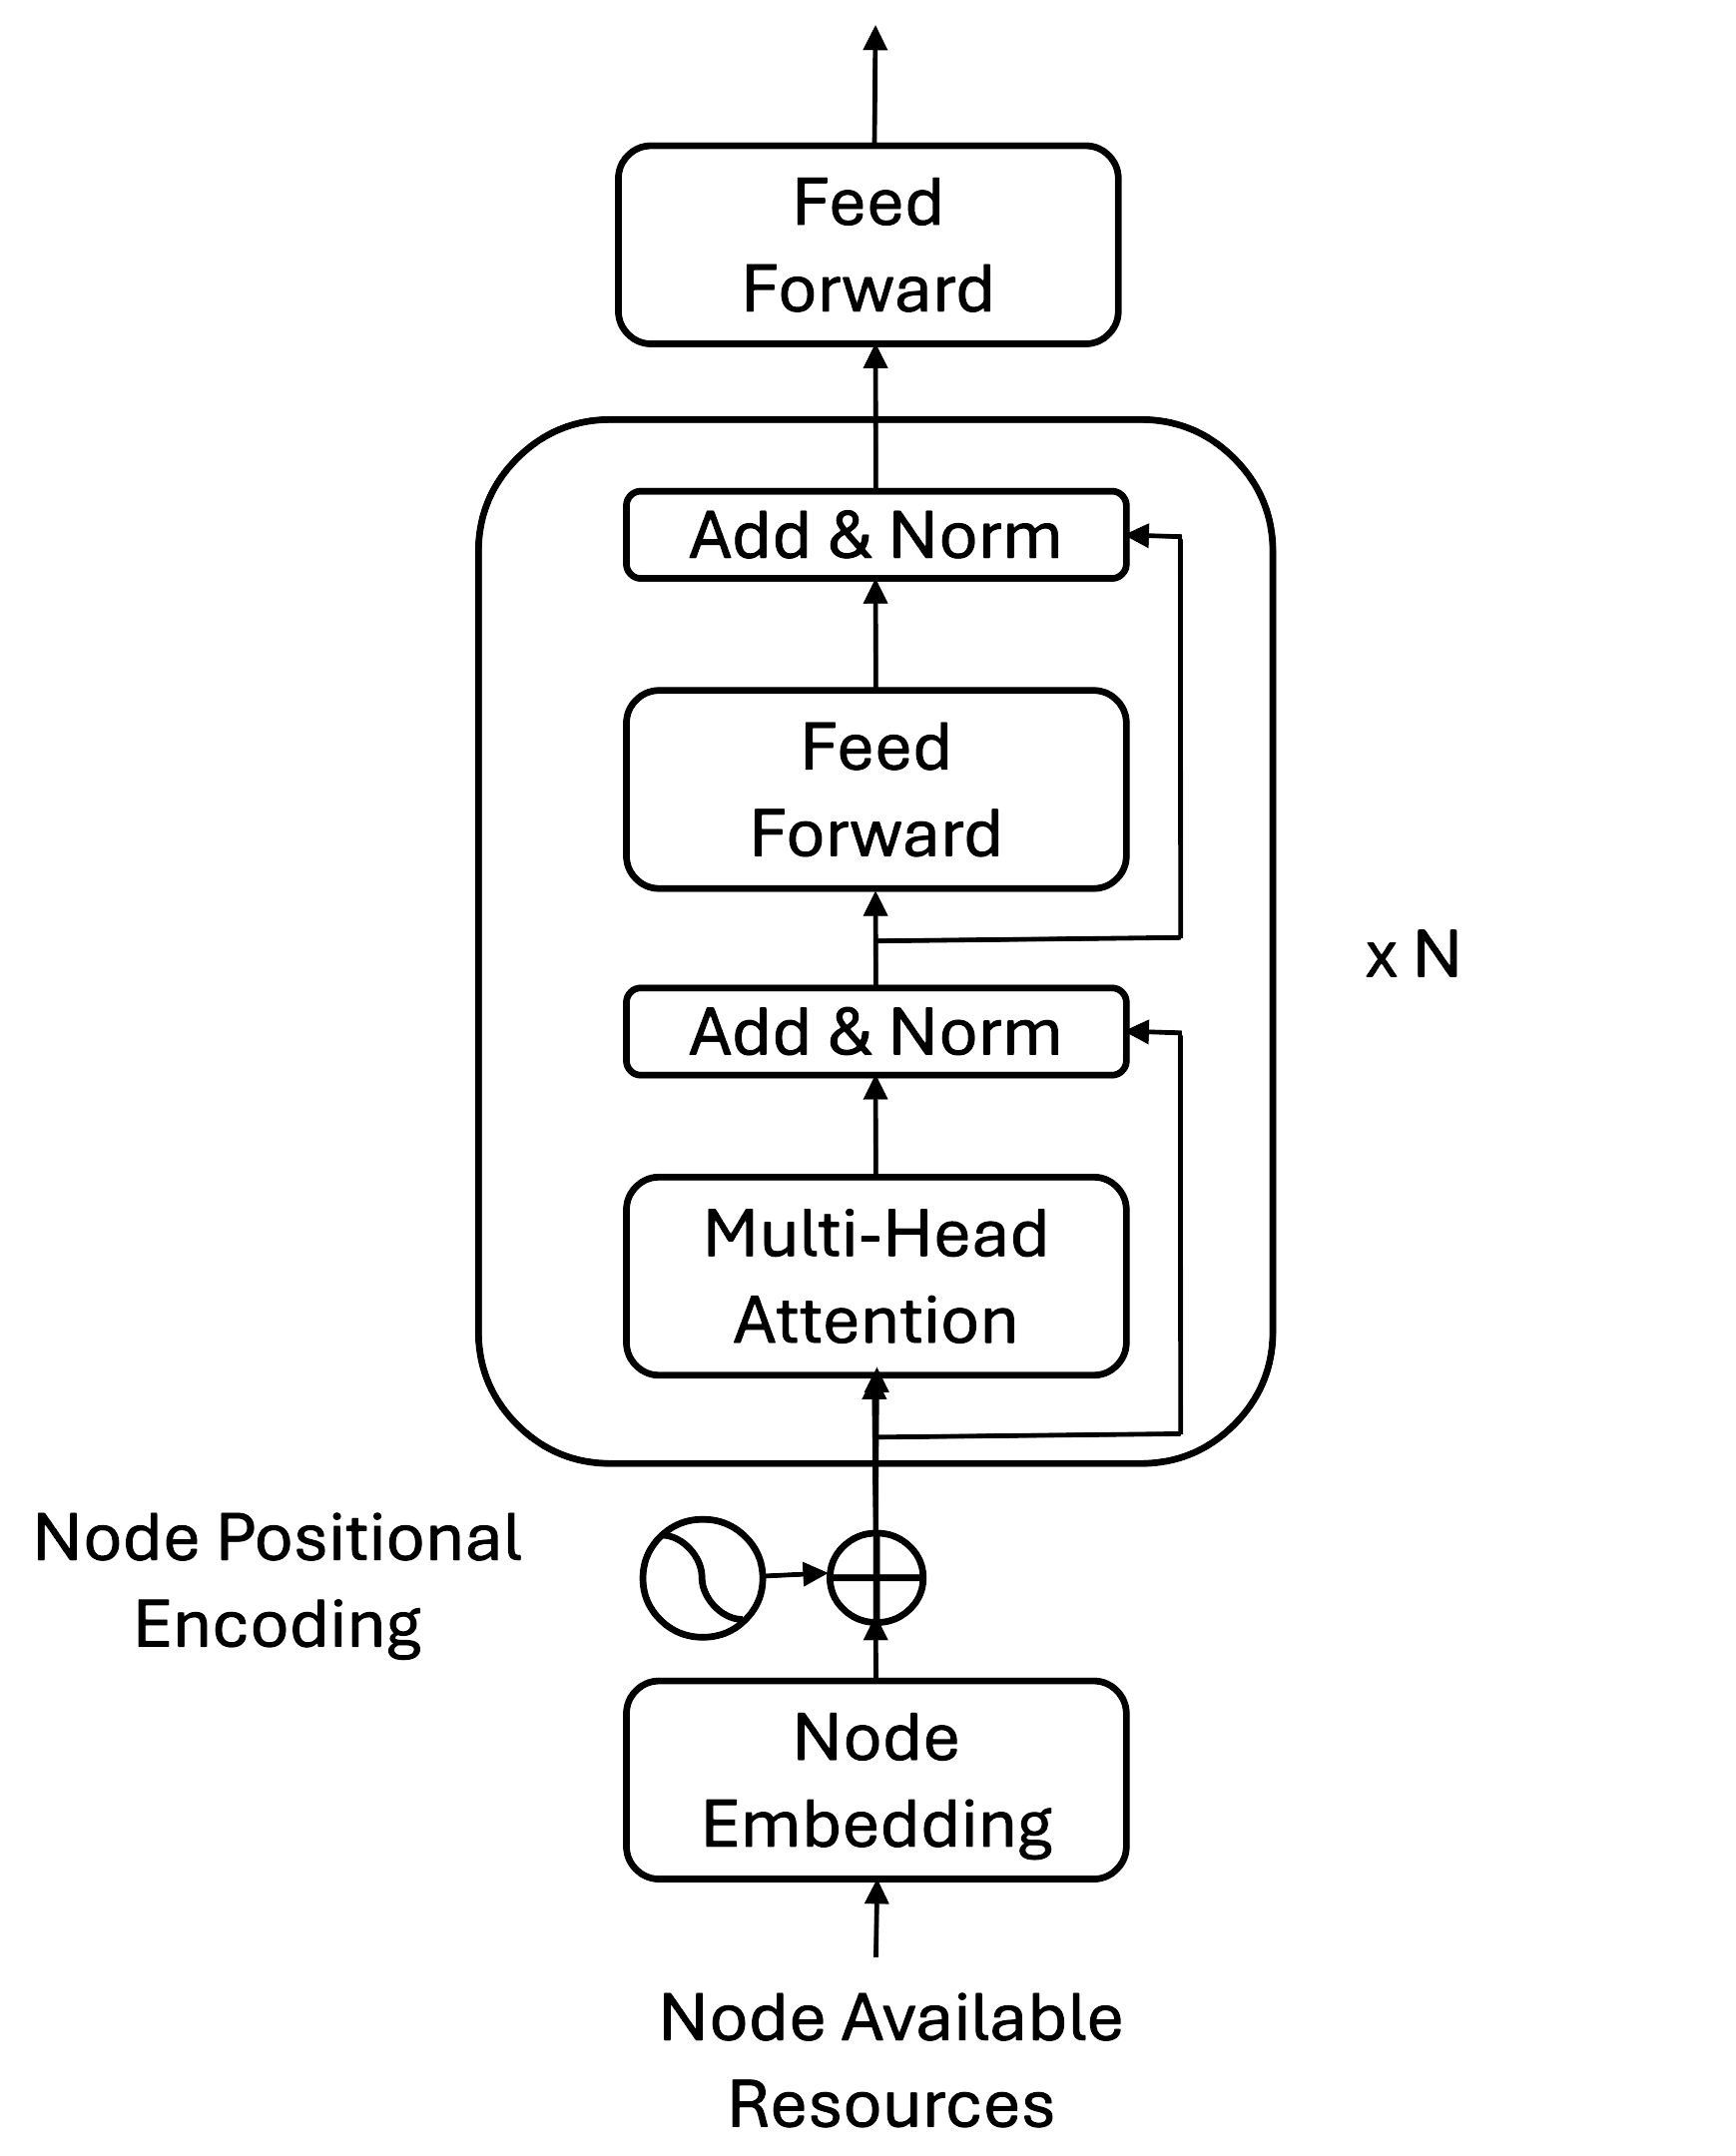
\includegraphics[width=0.6\linewidth]{figs/nodeformer_architecture.png}
    \caption{NOTE Architecture}\label{fig:note_architecture}
\end{figure}

\paragraph{T-NOTE}\label{par:T-NOTE}

T-NOTE extends NOTE by incorporating task attributes (e.g., size, deadline, and CPU-cycle requirements). These task features are passed through a fully connected layer to produce a vector of size \(d_{\text{model}}\). The resulting vector is then replicated across the \(n_{\text{nodes}}\) dimension and added to the node embeddings and node positional encodings before entering the Transformer encoder. Task-specific positional encoding can be combined or managed separately, allowing the model to capture task characteristics through shared attention. While including task information enables the Transformer encoder to more accurately learn interactions between node resources and task demands, it also increases the complexity of each DQL state. This added complexity sometimes leads to greater model instability, as rapid changes in the task dimension can cause oscillations in policy behavior. Consequently, NOTE (which omits explicit task embeddings) may remain advantageous in scenarios where a simpler, more stable representation is desired.


\begin{figure}[H]
    \centering
    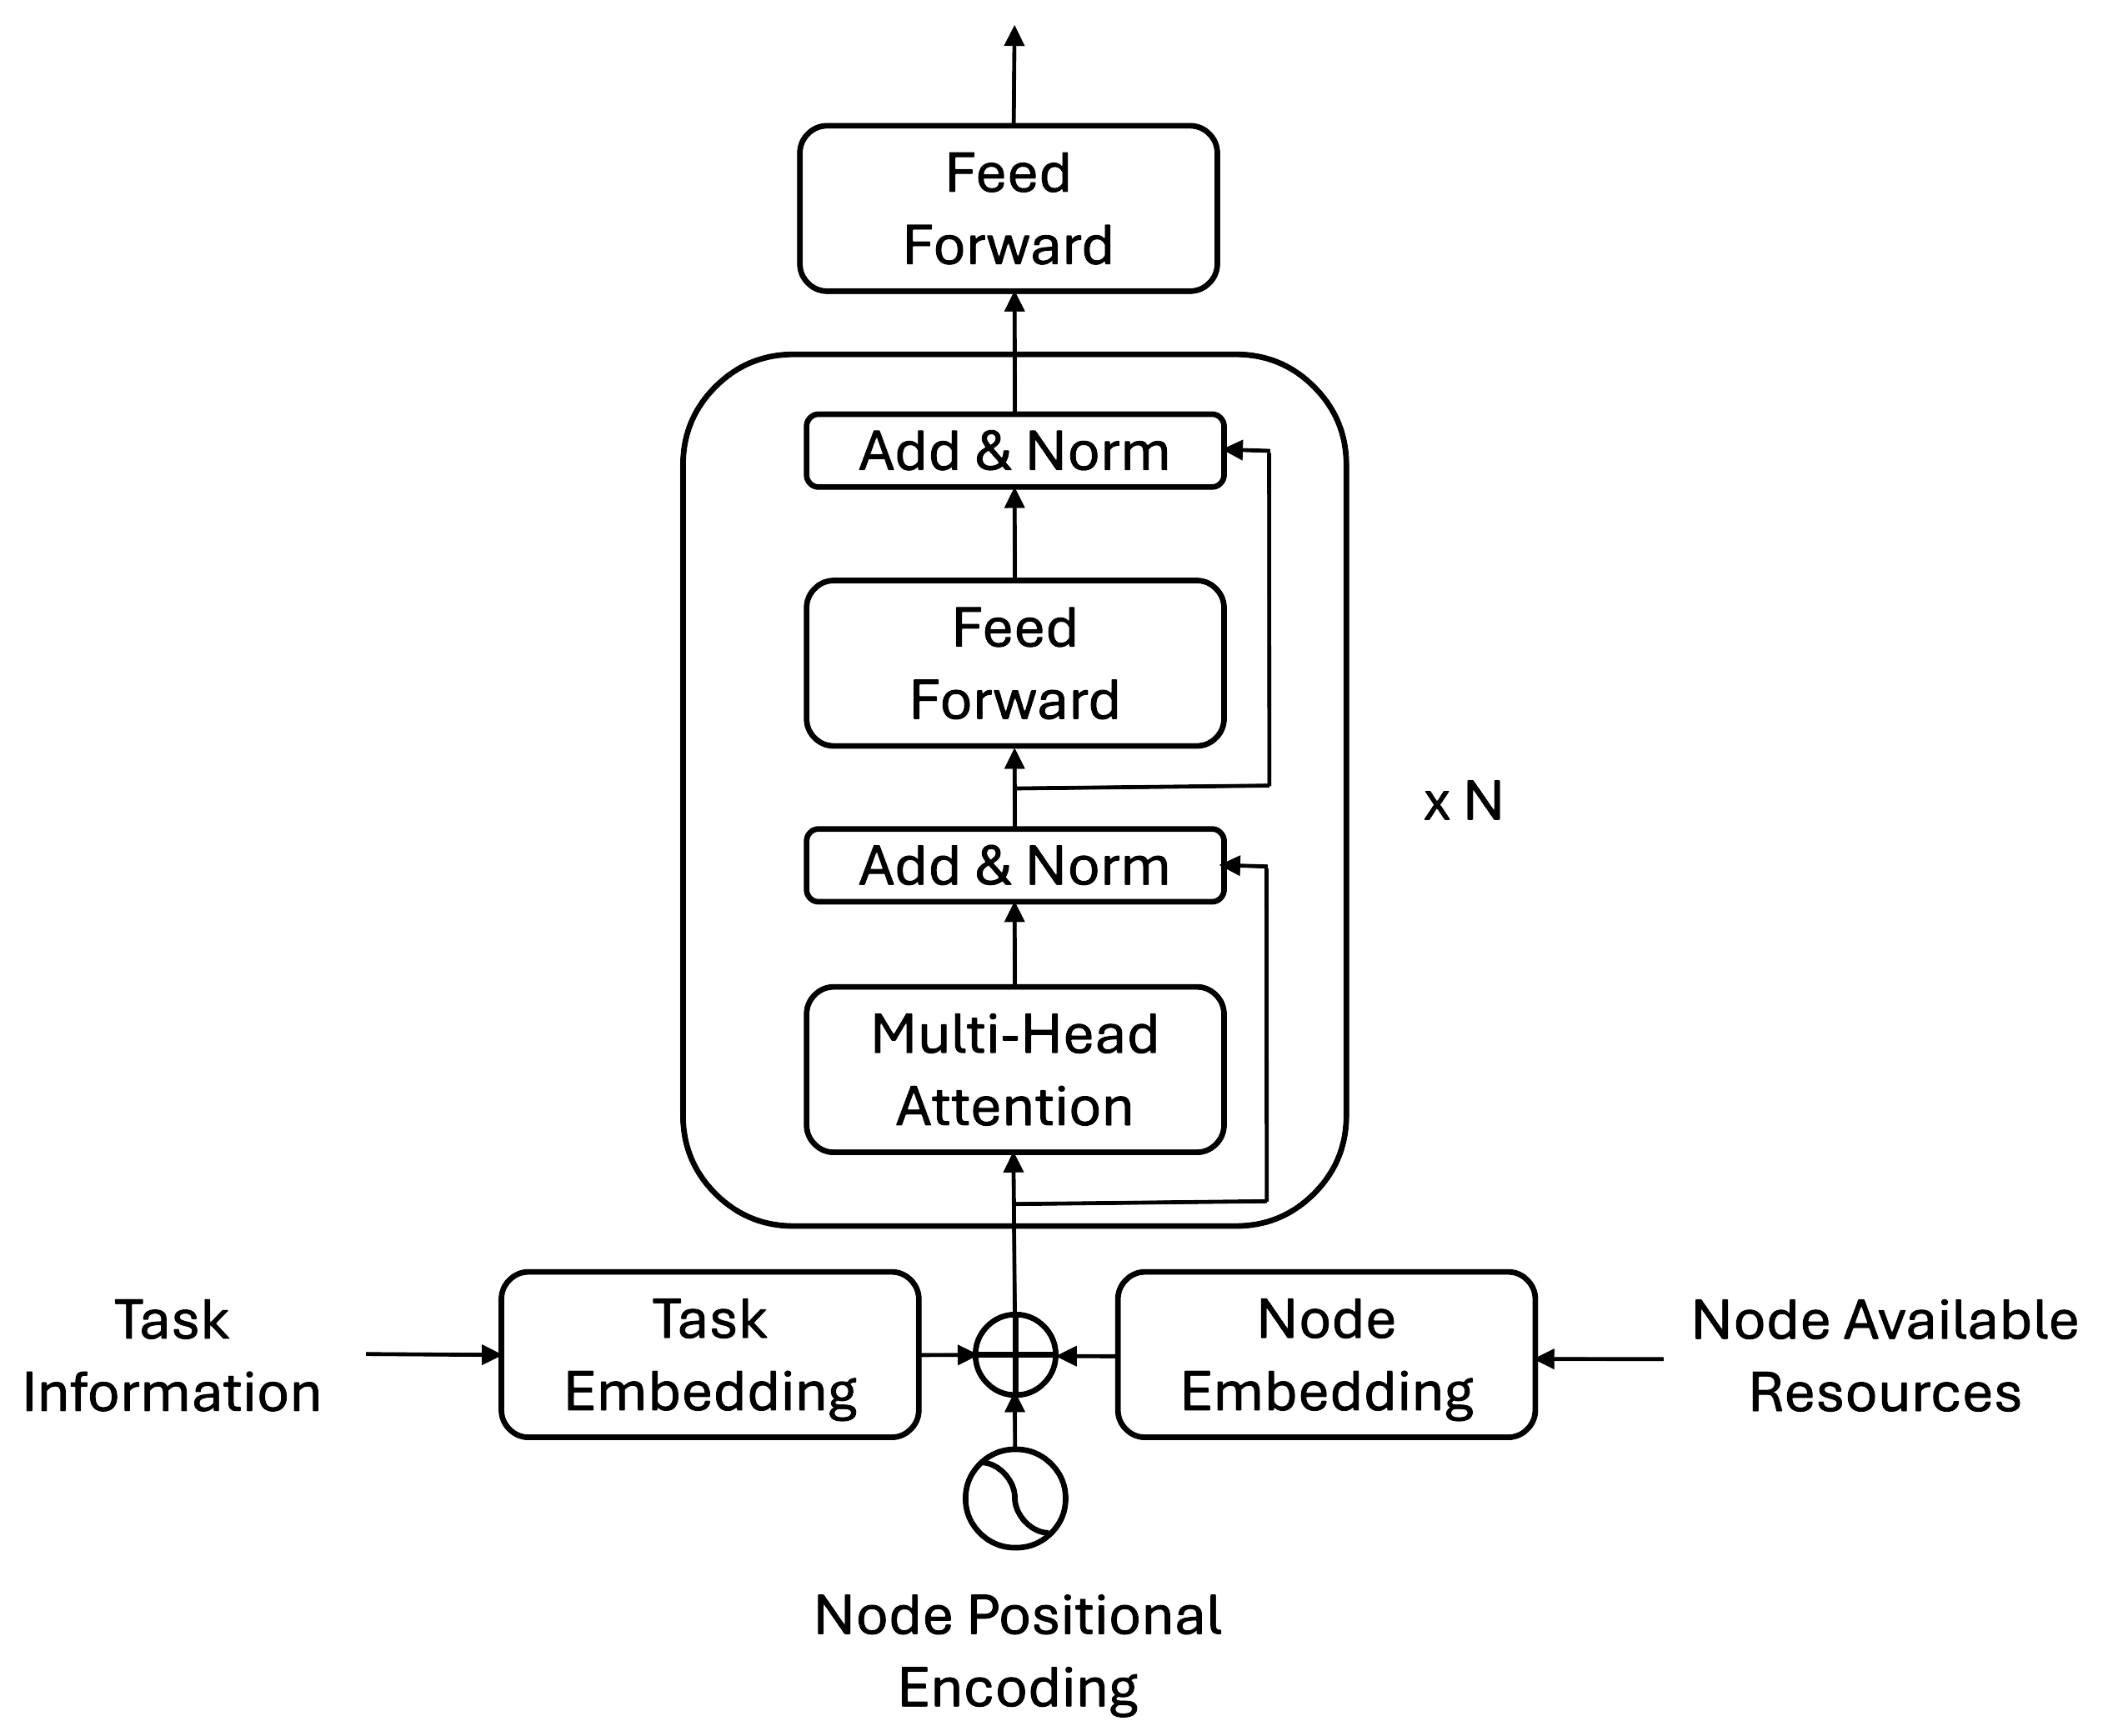
\includegraphics[width=0.8\linewidth]{figs/taskformer_architecture.png}
    \caption{T-NOTE Architecture}\label{fig:t-note_architecture}
\end{figure}


\begin{algorithm}[H]
\caption{Deep Q-Reinforcement Learning for IoT Task Offloading}\label{alg:DQL_iot_offloading}
\begin{algorithmic}[1]
\REQUIRE{Environment $\mathcal{E}$, task dataset $\mathcal{D}$, hyperparameters $\{\alpha, \gamma, \epsilon_0, \epsilon_{\text{decay}}, \lambda_0, \lambda_1, \lambda_2\}$}
\ENSURE{Trained Q-network policy $\pi^*$}

\STATE{Initialize Q-network $Q_\theta$ with random parameters $\theta$}
\STATE{Initialize experience replay buffer $\mathcal{B} \leftarrow \emptyset$}
\STATE{Set exploration rate $\epsilon \leftarrow \epsilon_0$}

\FOR{epoch $e = 1$ to $E_{\max}$}
    \STATE{Initialize epoch metrics: $L_{\max}^{(e)} \leftarrow 0$, $E_{\max}^{(e)} \leftarrow 0$}

    \FOR{each task $\tau_i \in \mathcal{D}$ ordered by generation time}
        \STATE{Wait until $t_{\text{current}} \geq \tau_i.\text{arrival\_time}$}
        \STATE{Construct state vector $s_i$ from system resources/task features}

        \STATE{\textbf{Action Selection:}} 
        \IF{$\text{rand}() < \epsilon$}
            \STATE{$a_i \leftarrow$ random edge node}
        \ELSE{}
            \STATE{$a_i \leftarrow \arg\max_{a} Q_\theta(s_i, a)$}
        \ENDIF{}
        
        \STATE{Execute offloading action $a_i$ and simulate task execution}
        \STATE{Observe next state $s_{i+1}$ and compute reward:}
        \STATE{
        \[
        r_i = -\begin{cases}
        \lambda_0 & \text{if task execution fails} \\[0.5em]
        \lambda_1 \cdot \frac{L_i}{L_{\max}^{(e)}} + \lambda_2 \cdot \frac{E_i}{E_{\max}^{(e)}} & \text{otherwise}
        \end{cases}
        \]
        }
        
        \STATE{Store transition $(s_i, a_i, r_i, s_{i+1})$ in $\mathcal{B}$}
        
        \IF{$|\mathcal{B}| \geq$ batch\_size \OR{} end of epoch}
            \STATE{Sample mini-batch $\mathcal{M}$ from $\mathcal{B}$}
            \FOR{each $(s, a, r, s') \in \mathcal{M}$}
                \STATE{Compute target: $y = r + \gamma \cdot \max_{a'} Q_\theta(s', a')$}
            \ENDFOR{}
            \STATE{Update Q-network: $\theta \leftarrow \theta - \alpha \nabla_\theta \mathcal{L}(\theta)$}
            \STATE{where $\mathcal{L}(\theta) = \mathbb{E}_{(s,a,r,s') \sim \mathcal{M}} \big[{(Q_\theta(s,a) - y)}^2\big]$}
            \STATE{Decay exploration: $\epsilon \leftarrow \epsilon \cdot \epsilon_{\text{decay}}$}
        \ENDIF{}
    \ENDFOR{}
\ENDFOR{}





\RETURN{Optimal policy $\pi^*(s) = \arg\max_a Q_\theta(s,a)$}
\end{algorithmic}
\end{algorithm}

\section{Performance Evaluation}\label{sec:performance_evaluation}

\subsection{Experimentation Setup}

T-NOTE is trained on a workstation equipped with a 16-core CPU, 64 GB of RAM, and an NVIDIA Tesla P100 GPU with 16 GB of memory. This configuration provides sufficient computational power to accelerate neural network training on large batches.


\subsubsection{Dataset}\label{subsec:dataset}

A real IoT task trace collected in Islamabad, Pakistan, is utilized as described by~\cite{aazam_cloud_2022}. This dataset contains heterogeneous IoT jobs (commonly referred to as \emph{tuples}).

The dataset covers diverse devices (sensors, dumb objects, mobiles, actuators, and location-based nodes). Originally, data are sampled every minute over a one-hour period. To avoid clustering all tasks within the same second of each minute, tasks are uniformly distributed across that minute, producing a more realistic workload. The statistics of these tasks are reported in Table~\ref{tab:task-statistics}.



\begin{table*}[h!]
\centering

\resizebox{\columnwidth}{!}{%
\begin{tabular}{|l|c|c|c|c|c|}
\hline
\textbf{Statistic} & \textbf{Generation Time (s)} & \textbf{Task Size (MB)} & \textbf{Cycles/Bit} & \textbf{Trans. Bit Rate (MB/s)} & \textbf{DDL (s)} \\ \hline
Count & 30,000 & 30,000 & 30,000 & 30,000 & 30,000 \\ \hline
Mean & 1891 & 206 & 344 & 88 & 60 \\ \hline
Std Dev & 1094 & 75 & 351 & 39 & 23 \\ \hline
Min & 0 & 80 & 50 & 20 & 20 \\ \hline
25\% & 941 & 170 & 100 & 80 & 39 \\ \hline
50\% & 1884 & 220 & 200 & 90 & 60 \\ \hline
75\% & 2856 & 270 & 700 & 100 & 79 \\ \hline
Max & 3780 & 300 & 1200 & 150 & 99 \\ \hline
\end{tabular}%
}
\caption{Statistical Summary of Generated Tasks}\label{tab:task-statistics}
\end{table*}


This dataset is adapted for the RayCloudSim framework, retaining only the most pertinent variables and appending additional information (for example, the number of cycles per bit). The units—originally unspecified in the source—are standardized to align with typical IoT node specifications, thereby ensuring consistency and accuracy in subsequent simulations and experiments.

\subsubsection{System Resources and Topology}\label{subsec:system_resources_topology}

To align with the dataset location, we designate the GG in Islamabad, Pakistan as the Edge node. The Fog nodes are configured as Micro-Data Centers (MDCs) distributed across various cities in Pakistan to provide regional computational resources. For the Cloud layer, we select data centers based on Google's global data center locations \citep{googleDataCenters}, specifically choosing the geographically nearest data centers to Pakistan to minimize latency overhead and ensure realistic network conditions.


In Figure~\ref{fig:used_architecture}, a network is shown to consist of eight nodes (\textit{Edge}, \textit{Fog}, and \textit{Cloud}) connected by multiple links with diverse bandwidth capacities. The \textit{edge node} (\texttt{e0}) is equipped with a low CPU frequency and a limited task buffer, whereas the \textit{fog nodes} (\texttt{f0}, \texttt{f1}, \texttt{f2}, \texttt{f3}, \texttt{f4}) has intermediate CPU frequencies and queue sizes. The \textit{cloud nodes} (\texttt{c0}, \texttt{c1}) exhibits the highest CPU frequencies and large buffer capacities, although they may incur higher idle power consumption and larger network latency due to their remote location.

\begin{figure}[H]
    \centering
    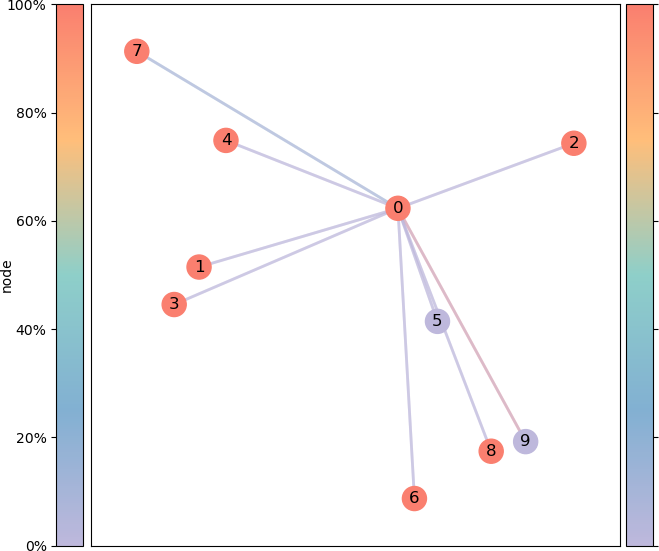
\includegraphics[width=0.75\linewidth]{figs/used_architecture.png}
    \caption{Used Architecture featuring Edge (Global Gateway), Fog (MDCs), and Cloud.}\label{fig:used_architecture}
\end{figure}


In Table~\ref{tab:node-specifications}, node specifications are listed, including Millions of Instructions Per Second (MIPS) which is the CPU frequency, the buffer size in GB, the up and down bandwidth from/to e0 (the global gateway) in GB and power coefficients in W. The network links range from 700 bps to 50,000 bps, forming a heterogeneous environment suitable for analyzing resource allocation and routing strategies under variable link constraints.


\begin{table*}[h!]
\centering

\resizebox{\columnwidth}{!}{%
\begin{tabular}{|l|c|c|c|c|c|c|c|c|l|}
\hline
\textbf{Node} & \textbf{Type} & \textbf{ID} & \textbf{MIPS} & \textbf{Buffer} & \textbf{Up BW} & \textbf{Down BW} & \textbf{Idle P} & \textbf{Exec P} & \textbf{Location} \\
\hline
e0 & Edge & 0 & 10 & 4 & -- & -- & 3 & 10 & Islamabad, PK \\ \hline
f0 & Fog & 1 & 110 & 16 & 2.5 & 1.7 & 30 & 150 & Multan, PK \\ \hline
f1 & Fog & 2 & 50 & 6 & 1 & 700 & 15 & 50 & Gilgit, PK \\ \hline
f2 & Fog & 3 & 95 & 12 & 2 & 1.5 & 25 & 120 & Karachi, PK \\ \hline
f3 & Fog & 4 & 85 & 10 & 1.5 & 1.2 & 20 & 100 & Lahore, PK \\ \hline
f4 & Fog & 5 & 75 & 8 & 1.2 & 1 & 20 & 100 & Peshawar, PK \\ \hline
c0 & Cloud & 6 & 500 & 51 & 3 & 3 & 300 & 1100 & Singapore \\ \hline
c1 & Cloud & 7 & 500 & 51 & 3 & 3 & 250 & 1000 & Belgium \\ \hline
\end{tabular}%
}
\caption{Detailed Specifications of Nodes}\label{tab:node-specifications}
\end{table*}


\subsection{Hyperparameters}\label{subsec:hyperparameters}


Since our modeling framework assigns zero latency and energy values to tasks that fail to be successfully offloaded, the primary optimization objective becomes the minimization of the \emph{task throw rate}. This constraint is essential to prevent model degeneration, where the system could exploit the null assignment by deliberately rejecting tasks to artificially improve energy and latency performance metrics.

To enhance the stability of the optimization process, a hierarchical prioritization scheme has been adopted, with a greater emphasis on latency in comparison to energy efficiency. This is due to the fact that latency exerts a more direct influence on both the user experience and the system's responsiveness. This prioritization is reflected in the reward weight hierarchy:

\[
\lambda_0 \gg \lambda_1 > \lambda_2.
\]

Based on empirical evaluation of different configurations using a MLP architecture trained with DQL, we selected the following reward weight distribution:

\[
\textbf{Reward weights } (\lambda) = [1,\; 0.1,\; 0.05].
\]


\subsubsection{Model Configurations}

The complete hyperparameter specifications are detailed in Table~\ref{tab:model_specifications}. These specifications guide the architecture and training of both the MLP and Transformer models under the DQL algorithm. Feature used as input include task attributes for T-models.


\begin{table}[H]
\centering

\resizebox{\columnwidth}{!}{%
\begin{tabular}{|l|c|c|}
\hline
\textbf{Parameter} & \textbf{Transformer Model} & \textbf{MLP Model} \\ \hline
Hidden dimension ($d_{\text{model}}$) & 64 & 256 \\ \hline
Number of layers ($n_{\text{layers}}$) & 6 & 3 \\ \hline
Number of heads ($n_{\text{heads}}$) & 4 & - \\ \hline
Feed Forward Network ($d_{\text{ff}}$) & 256 & - \\ \hline
Dropout & 0.2 & 0 \\ \hline
Activation function & GELU & ReLU \\ \hline
Input features & \{cpu, bw, buffer\} + \{task\_type\}  \\ \hline
\end{tabular}%
}
\caption{Model Specifications}\label{tab:model_specifications}
\end{table}

\subsubsection{Heuristic Baseline Methods}\label{subsubsec:heuristic_baselines}
We implement baseline heuristic approaches for comparative evaluation, namely, \emph{Random}, \emph{Round Robin (RR)} and \emph{Greedy}.

\paragraph{Random}
Random strategy, consist to randomly assign tasks to nodes uniformly at random, without consideration of current resource availability or node capabilities.

\paragraph{Round Robin}
RR is a straightforward load balancing technique where tasks are cyclically distributed among nodes, with each node receiving tasks in turn before cycling back to the first node. This ensures basic load balancing but ignores node heterogeneity such as CPU frequencies and buffer sizes, potentially causing inefficiencies under varied workloads. 

\paragraph{Greedy}
Greedy methods assign tasks based on immediate resource availability or specific cost metrics, such as selecting the node with the highest remaining CPU capacity. While easily implemented and computationally efficient, greedy strategies often forgo long-term, globally optimal decisions in favor of immediate local optima.




\subsection{Convergence Analysis}

The NOTE architecture encodes exclusively node-level features (CPU availability, buffer capacity, and bandwidth), aggregated across tasks. As illustrated in Figure~\ref{fig:NOTE-score-plot}, the learning process rapidly stabilizes and converges at epoch 4, where the optimal model is selected. This expedited convergence demonstrates the effectiveness of self-attention mechanisms in capturing and refining multi-node relationships.

\begin{figure}[H]
    \centering
    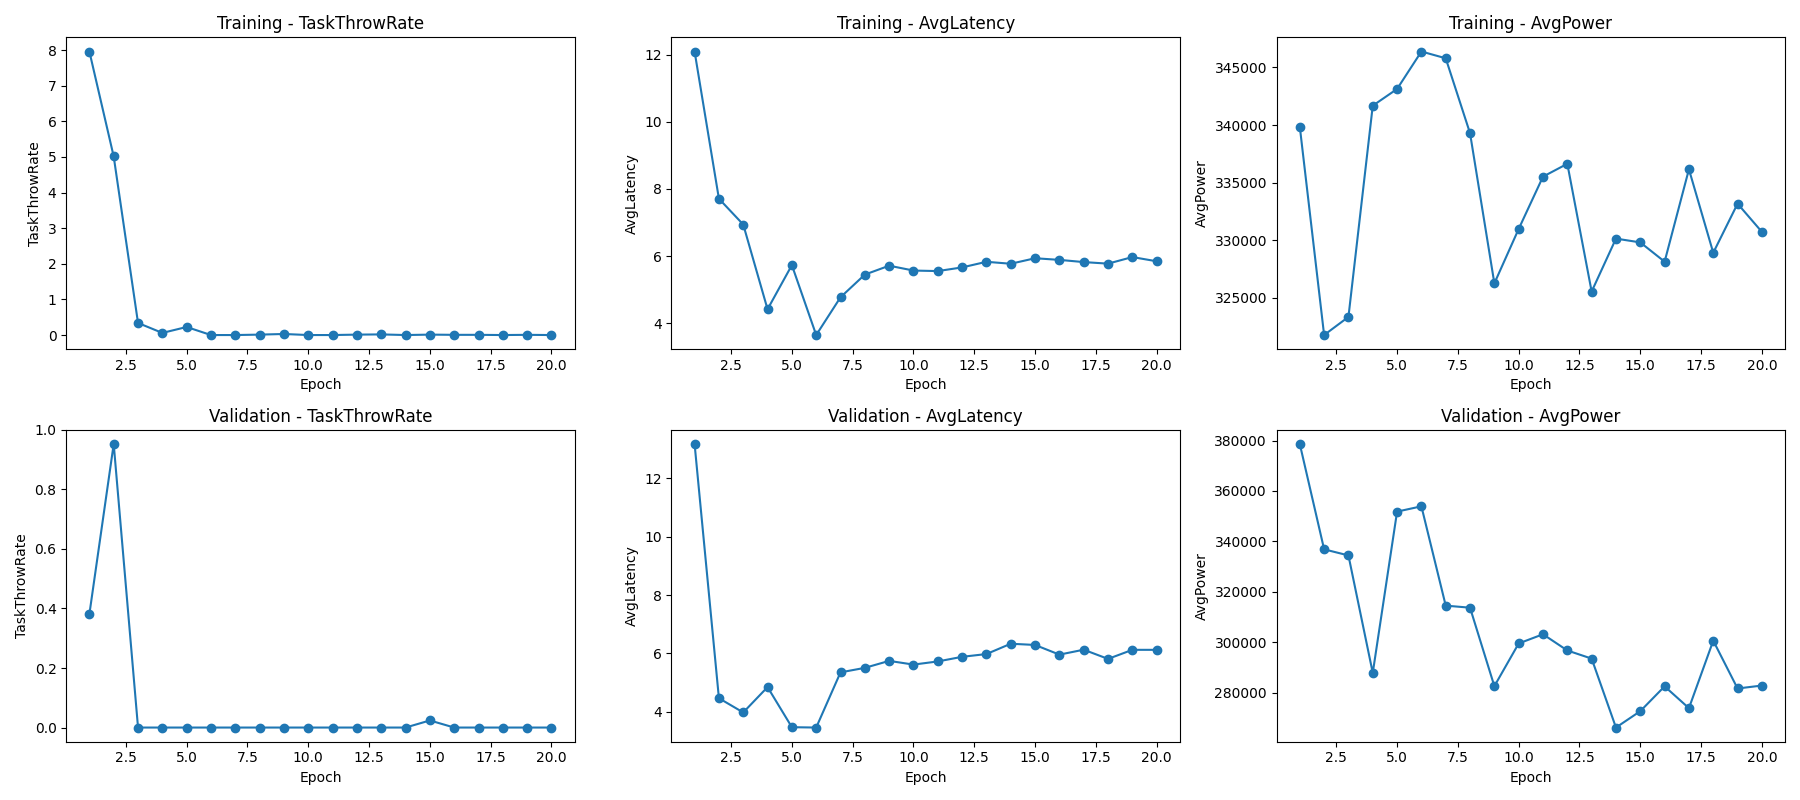
\includegraphics[width=1\linewidth]{figs/NOTE/score_plot.png}
    \caption{Training convergence and performance scores for NOTE-based DQL approach.}
    \label{fig:NOTE-score-plot}
\end{figure}

However, performance degradation occurs after epoch 4, potentially indicating convergence to a local optimum. This behavior suggests that while NOTE efficiently learns effective offloading policies, it may benefit from additional exploration strategies or more expressive feature representations. The incorporation of task-level features in T-NOTE effectively addresses this limitation.

The additional features, added by the task-level attributes, enable more contextually informed offloading decisions, resulting in improved convergence characteristics and superior performance with respect to both latency and task success rate. Figure~\ref{fig:T-NOTE-score-plot} demonstrates the convergence behavior of T-NOTE throughout the training process.

\begin{figure}[H]
    \centering
    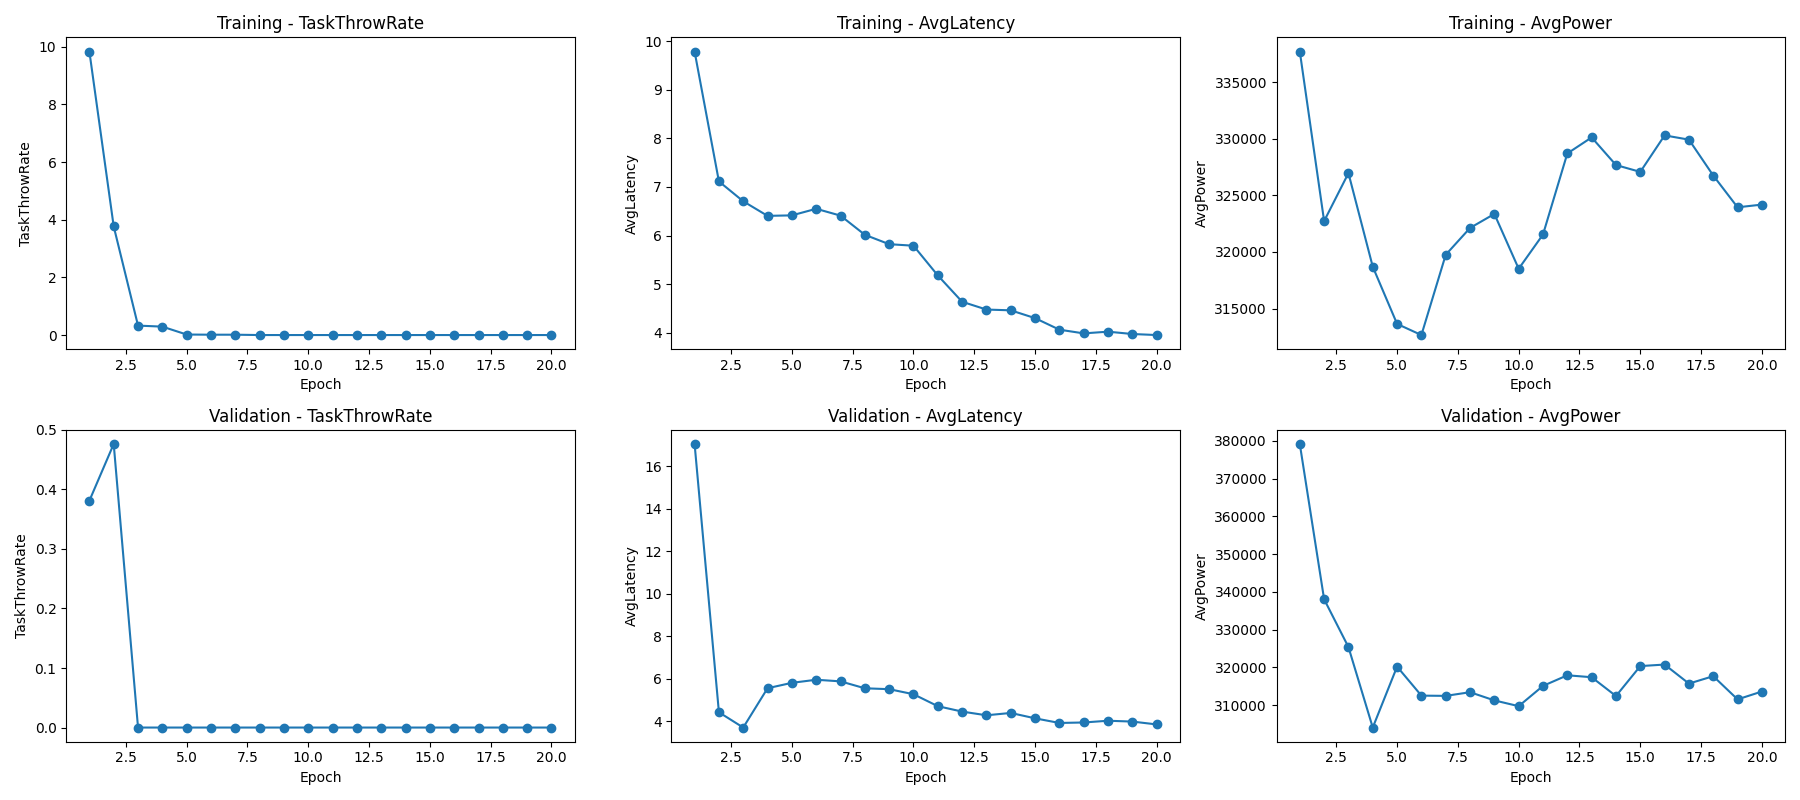
\includegraphics[width=1\linewidth]{figs/T-NOTE/score_plot.png}
    \caption{Training convergence and performance scores for T-NOTE-based DQL approach.}
    \label{fig:T-NOTE-score-plot}
\end{figure}

Similar to NOTE, T-NOTE exhibits rapid score improvement during the initial epoch, reflecting quick adaptation to the task offloading problem. However, unlike NOTE, which experiences performance degradation after epoch 4, T-NOTE demonstrates continued exploration capabilities. The score exhibits a secondary descent from epoch 16 through the final training epoch. This behavior indicates that the model continues to refine its policy in pursuit of improved solutions, suggesting that the task-aware attention mechanism provides sufficient representational capacity to avoid premature convergence to local optima. This sustained exploration capability, combined with the model's ability to leverage task-specific information, enables T-NOTE to discover superior offloading strategies that achieve the best overall performance across all evaluation metrics during the test, as demonstrated in Table~\ref{tab:results_comparison}.
\subsection{Evaluation}

The evaluation of heuristic baseline methods reveals a fundamental trade-off between energy efficiency and performance, allowing us to categorize offloading strategies into two distinct classes: (i) \emph{energy-centric} strategies (\emph{Random} and \emph{Round Robin}), which prioritize energy efficiency at the cost of elevated task failure rates and increased latency; and (ii) \emph{performance-centric} strategies (\emph{Greedy}), which substantially reduce task failures and latency while consuming more energy.


To evaluate the flexibility of the proposed DRL-based approach with respect to energy optimization, we compare T-NOTE against energy-centric heuristic baselines (Random and Round Robin) under appropriately adjusted reward weights that prioritize energy efficiency. Table~\ref{tab:energy_comparison} presents these results.

\begin{table*}[htbp]
\centering
\begin{tabular}{lccc}
\toprule
\textbf{Offloading Strategy} & \textbf{TTR (\%)} & \textbf{Latency (s)} & \textbf{Energy (W)} \\
\midrule
Random 
 & 14.21
 & 20.89
 & 238.3 \\
Round Robin 
 & 14.98
 & 18.36
 & 239.9 \\
\midrule
T-NOTE (energy-optimized)
 & \textbf{0.3556} 
 & \textbf{5.976} 
 & \textbf{238.0} \\
\bottomrule
\end{tabular}
\caption{Performance comparison of T-NOTE with energy-optimized reward weights against heuristic baselines on the Pakistan test set. Best results are shown in \textbf{bold}.}
\label{tab:energy_comparison}
\end{table*}

The heuristic baselines exhibit TTRs exceeding 14\% and latencies above 18 seconds. These poor performance characteristics stem from their simplistic task assignment mechanisms, which distribute tasks uniformly without consideration of node resource capacities. While this approach achieves low energy consumption (approximately 239~W) by utilizing a larger number of fog nodes~\ref{subsec:random}, it fundamentally fails to meet performance requirements.

In contrast, the Greedy approach achieves a TTR of 0.1889\% and latency of 4.394 seconds by preferentially selecting nodes with the highest available CPU resources~\ref{subsec:greedy-baseline}, but increased energy consumption (338.7~W). This leads to the classification of performance-centric strategies.

When configured with energy-optimized reward weights, T-NOTE achieves a TTR approximately 40 times lower and latency approximately 3.5 times lower than the heuristic baselines, while maintaining comparable energy consumption (238.0~W). This result demonstrates that T-NOTE can be effectively adapted to diverse optimization objectives through reward weight configuration, highlighting both the effectiveness and flexibility of the proposed DRL-based approach for task offloading in hierarchical edge-fog-cloud environments.

\subsection{Offloading Analysis}\label{subsec:offloading-analysis}

This section analyzes the offloading strategies employed by different approaches, examining their performance characteristics, resource utilization patterns, and trade-offs. The analysis provides insights into how each method addresses task allocation challenges in hierarchical edge-fog-cloud computing environments.

\begin{figure}[H]
    \centering
    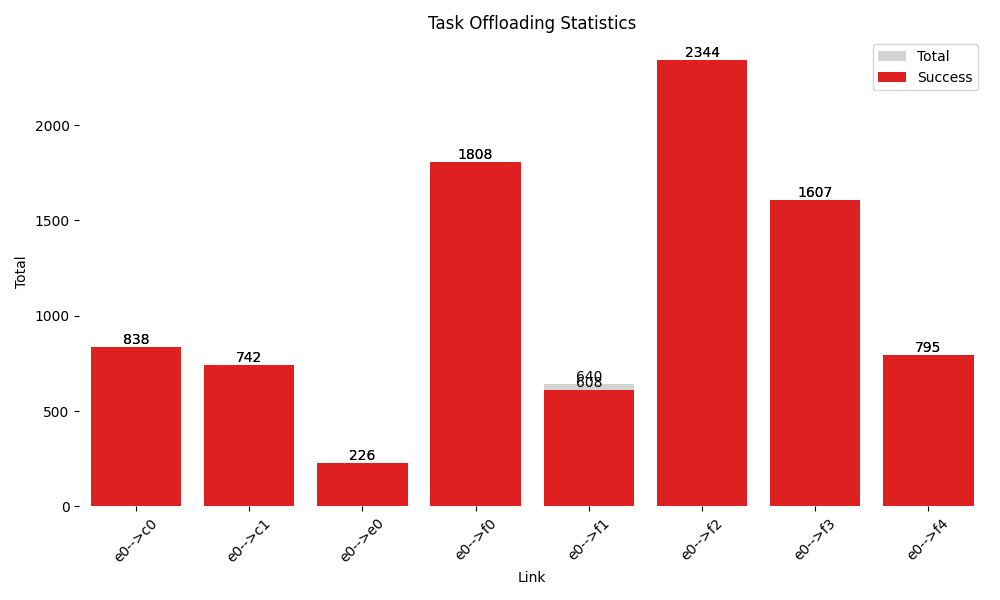
\includegraphics[width=0.5\linewidth]{figs/T-NOTE4E/task_offloading_statistics.png}
    \caption{Task offloading distribution for T-NOTE}
    \label{fig:T-NOTE-offloading-stats}
\end{figure}


\section{Conclusion and Perspectives}\label{sec:conclusion}

This work addresses the critical challenge of task offloading in hierarchical edge-fog-cloud computing environments through a comprehensive investigation of metaheuristic and deep reinforcement learning approaches. A realistic evaluation framework is established using real IoT task traces from Pakistan, integrated within the RayCloudSim simulation platform, and made publicly available to facilitate reproducible research and community advancement.

The proposed NOTE and T-NOTE architectures demonstrate the effectiveness of Transformer-based approaches for task offloading optimization. T-NOTE, which incorporates both node-level and task-level observations through attention mechanisms, achieves superior performance across all evaluated metrics compared to baseline methods. Specifically, T-NOTE eliminates task failures entirely (0\% TTR) while achieving 16.6\% lower latency and 6.4\% reduced energy consumption compared to the Greedy baseline. These results underscore the value of attention mechanisms in capturing complex relationships between heterogeneous node resources and diverse task requirements.

The comparative analysis between genetic algorithms and deep Q-learning reveals complementary strengths. Multi-objective GA methods (NSGA-II, NPGA) successfully generate diverse Pareto-optimal solution sets, providing practitioners with flexible trade-off options among competing objectives. However, these methods incur substantial computational overhead due to population-based evaluation across multiple generations. In contrast, DQL-based approaches demonstrate faster convergence and lower computational requirements while achieving competitive performance, making them particularly suitable for scenarios requiring rapid deployment and real-time adaptation.

The experimental results highlight that task-aware Transformer architectures can effectively balance multiple competing objectives—latency minimization, energy efficiency, and reliability—through appropriate reward weight tuning. The demonstrated flexibility of T-NOTE in adapting to different optimization priorities (as shown in the energy consideration experiments) validates the practical applicability of the proposed approach across diverse deployment scenarios and operational requirements.

\subsection{Perspectives}


\paragraph{Reward weights tuning}

Automatically tuning the reward weights would be a significant improvement to the DQL approach. This could involve meta-learning techniques or adaptive weight adjustment based on observed performance metrics during training. Automating this process would reduce the reliance on manual tuning and enhance the robustness of the offloading strategy across varying scenarios.


\paragraph{Advanced Reinforcement Learning Architectures}
Future work should explore policy gradient methods such as Proximal Policy Optimization (PPO), Advantage Actor-Critic (A2C), and Deep Deterministic Policy Gradient (DDPG), which may offer improved stability and sample efficiency compared to value-based DQL approaches.


\paragraph{Multi-Objective Optimization}
A more extensive investigation of multi-objective genetic algorithms could provide valuable insights into the trade-offs between different QoS metrics. Developing lightweight variants of GA suitable for high-dimensional parameter spaces would enable the discovery of comprehensive Pareto frontiers for complex neural architectures.

%
% ---- Bibliography ----
%


\begin{thebibliography}{99}

\bibitem{mishra_collaborative_2023}
Mishra, K., Rajareddy, G.N.V., Ghugar, U., Chhabra, G.S., Gandomi, A.H.: A Collaborative Computation and Offloading for Compute-Intensive and Latency-Sensitive Dependency-Aware Tasks in Dew-Enabled Vehicular Fog Computing: A Federated Deep Q-Learning Approach. IEEE Transactions on Network and Service Management 20(4), 4600--4614 (2023). \url{https://doi.org/10.1109/TNSM.2023.3282795}

\bibitem{benaboura_comprehensive_nodate}
Benaboura, A., Bechar, R., Kadri, W.: A comprehensive survey of task offloading techniques in IoT-Fog-Cloud computing

\bibitem{alsadie_advancements_2024}
Alsadie, D.: Advancements in heuristic task scheduling for IoT applications in fog-cloud computing: challenges and prospects. PeerJ Computer Science 10, e2128 (2024). \url{https://doi.org/10.7717/peerj-cs.2128}

\bibitem{jeyaraman_applications_2024}
Jeyaraman, N., Jeyaraman, M., Yadav, S., Ramasubramanian, S., Balaji, S., Muthu, S., Lekha P, C., Patro, B.P.: Applications of Fog Computing in Healthcare. Cureus (2024). \url{https://doi.org/10.7759/cureus.64263}

\bibitem{fahimullah_review_2022}
Fahimullah, M., Ahvar, S., Trocan, M.: A Review of Resource Management in Fog Computing: Machine Learning Perspective. arXiv:2209.03066 [cs] (2022). \url{https://doi.org/10.48550/arXiv.2209.03066}

\bibitem{das_review_2023}
Das, R., Inuwa, M.M.: A review on fog computing: Issues, characteristics, challenges, and potential applications. Telematics and Informatics Reports 10, 100049 (2023). \url{https://doi.org/10.1016/j.teler.2023.100049}

\bibitem{penglin_survey_2024}
Penglin, D., Md Likhan: A Survey of Emerging Trends in Edge Computing. Unpublished (2024). \url{https://doi.org/10.13140/RG.2.2.22183.76962}

\bibitem{zhu_cloudfog_2024}
Zhu, C., Liu, C., Zhu, H., Li, J.: Cloud--Fog Collaborative Computing Based Task Offloading Strategy in Internet of Vehicles. Electronics 13(12), 2355 (2024). \url{https://doi.org/10.3390/electronics13122355}

\bibitem{wang_deep_2024}
Wang, Z., Goudarzi, M., Gong, M., Buyya, R.: Deep Reinforcement Learning-based scheduling for optimizing system load and response time in edge and fog computing environments. Future Generation Computer Systems 152, 55--69 (2024). \url{https://doi.org/10.1016/j.future.2023.10.012}

\bibitem{javaid_intelligent_2019}
Javaid, S., Javaid, N., Saba, T., Wadud, Z., Rehman, A., Haseeb, A.: Intelligent Resource Allocation in Residential Buildings Using Consumer to Fog to Cloud Based Framework. Energies 12(5), 815 (2019). \url{https://doi.org/10.3390/en12050815}

\bibitem{aazam_offloading_2018}
Aazam, M., Zeadally, S., Harras, K.A.: Offloading in fog computing for IoT: Review, enabling technologies, and research opportunities. Future Generation Computer Systems 87, 278--289 (2018). \url{https://doi.org/10.1016/j.future.2018.04.057}

\bibitem{yuan_online_2021}
Yuan, H., Tang, G., Li, X., Guo, D., Luo, L., Luo, X.: Online Dispatching and Fair Scheduling of Edge Computing Tasks: A Learning-Based Approach. IEEE Internet of Things Journal 8(19), 14985--14998 (2021). \url{https://doi.org/10.1109/JIOT.2021.3073034}

\bibitem{jiang_reinforcement_2021}
Jiang, F., Ma, R., Gao, Y., Gu, Z.: A reinforcement learning-based computing offloading and resource allocation scheme in F-RAN. EURASIP Journal on Advances in Signal Processing 2021(1), 91 (2021). \url{https://doi.org/10.1186/s13634-021-00802-x}

\bibitem{tu_task_2022}
Tu, Y., Chen, H., Yan, L., Zhou, X.: Task Offloading Based on LSTM Prediction and Deep Reinforcement Learning for Efficient Edge Computing in IoT. Future Internet 14(2), 30 (2022). \url{https://doi.org/10.3390/fi14020030}

\bibitem{gholipour_tpto_2023}
Gholipour, N., Assuncao, M.D., Agarwal, P., gascon-samson, j., Buyya, R.: TPTO: A Transformer-PPO based Task Offloading Solution for Edge Computing Environments. arXiv:2312.11739 [cs] (2023). \url{https://doi.org/10.48550/arXiv.2312.11739}

\bibitem{bukhari_intelligent_2022}
Bukhari, M.M., Ghazal, T.M., Abbas, S., Khan, M.A., Farooq, U., Wahbah, H., Ahmad, M., Adnan, K.M.: An Intelligent Proposed Model for Task Offloading in Fog-Cloud Collaboration Using Logistics Regression. Computational Intelligence and Neuroscience 2022, 1--25 (2022). \url{https://doi.org/10.1155/2022/3606068}

\bibitem{ometov_survey_2022}
Ometov, A., Molua, O., Komarov, M., Nurmi, J.: A Survey of Security in Cloud, Edge, and Fog Computing. Sensors 22(3), 927 (2022). \url{https://doi.org/10.3390/s22030927}

\bibitem{costa_orchestration_2023}
Costa, B., Bachiega, J., De Carvalho, L.R., Araujo, A.P.F.: Orchestration in Fog Computing: A Comprehensive Survey. ACM Computing Surveys 55(2), 1--34 (2023). \url{https://doi.org/10.1145/3486221}

\bibitem{wang_integration_nodate}
Wang, Z.: Integration of FogBus2 Framework with Container Orchestration Tools in Cloud and Edge Computing Environments

\bibitem{wali_anomaly_nodate}
Wali, G., Bulla, Dr C.: Anomaly Detection in Fog Computing: State-of-the-Art Techniques, applications, Challenges, and Future Directions

\bibitem{pakmehr_task_2024}
Pakmehr, A.: Task Offloading in Fog Computing with Deep Reinforcement Learning: Future Research Directions Based on Security and Efficiency Enhancements. arXiv:2407.19121 [cs] (2024). \url{https://doi.org/10.48550/arXiv.2407.19121}

\bibitem{jiang_delay_2018}
Jiang, Y., Tsang, D.H.K.: Delay-Aware Task Offloading in Shared Fog Networks. IEEE Internet of Things Journal 5(6), 4945--4956 (2018). \url{https://doi.org/10.1109/JIOT.2018.2880250}

\bibitem{iftikhar_ai_2023}
Iftikhar, S., Gill, S.S., Song, C., Xu, M., Aslanpour, M.S., Toosi, A.N., Du, J., Wu, H., Ghosh, S., Chowdhury, D., Golec, M., Kumar, M., Abdelmoniem, A.M., Cuadrado, F., Varghese, B., Rana, O., Dustdar, S., Uhlig, S.: AI-based Fog and Edge Computing: A Systematic Review, Taxonomy and Future Directions. Internet of Things 21, 100674 (2023). \url{https://doi.org/10.1016/j.iot.2022.100674}

\bibitem{guerrero_genetic_2022}
Guerrero, C., Lera, I., Juiz, C.: Genetic-based optimization in Fog Computing: current trends and research opportunities. Swarm and Evolutionary Computation 72, 101094 (2022). \url{https://doi.org/10.1016/j.swevo.2022.101094}

\bibitem{patel_navigating_nodate}
Patel, D.: Navigating Fog Federation: Classifying Current Research and Identifying Challenges

\bibitem{aazam_cloud_2022}
Aazam, M., Islam, S.U., Lone, S.T., Abbas, A.: Cloud of Things (CoT): Cloud-Fog-IoT Task Offloading for Sustainable Internet of Things. IEEE Transactions on Sustainable Computing 7(1), 87--98 (2022). \url{https://doi.org/10.1109/TSUSC.2020.3028615}

\bibitem{mcchesney_defog_2019}
McChesney, J., Wang, N., Tanwer, A., Lara, E.d., Varghese, B.: DeFog: Fog Computing Benchmarks. arXiv:1907.10890 [cs] (2019). \url{https://doi.org/10.48550/arXiv.1907.10890}

\bibitem{ren_deep_2021}
Ren, Y., Sun, Y., Peng, M.: Deep Reinforcement Learning Based Computation Offloading in Fog Enabled Industrial Internet of Things. IEEE Transactions on Industrial Informatics 17(7), 4978--4987 (2021). \url{https://doi.org/10.1109/TII.2020.3021024}

\bibitem{suryadevara_energy_2021}
Suryadevara, N.K.: Energy and latency reductions at the fog gateway using a machine learning classifier. Sustainable Computing: Informatics and Systems 31, 100582 (2021). \url{https://doi.org/10.1016/j.suscom.2021.100582}

\bibitem{adhikari_dpto_2020}
Adhikari, M., Mukherjee, M., Srirama, S.N.: DPTO: A Deadline and Priority-Aware Task Offloading in Fog Computing Framework Leveraging Multilevel Feedback Queueing. IEEE Internet of Things Journal 7(7), 5773--5782 (2020). \url{https://doi.org/10.1109/JIOT.2019.2946426}

\bibitem{yan_optimal_2020}
Yan, J., Bi, S., Zhang, Y.J., Tao, M.: Optimal Task Offloading and Resource Allocation in Mobile-Edge Computing With Inter-User Task Dependency. IEEE Transactions on Wireless Communications 19(1), 235--250 (2020). \url{https://doi.org/10.1109/TWC.2019.2943563}

\bibitem{jazayeri_autonomous_2021}
Jazayeri, F., Shahidinejad, A., Ghobaei-Arani, M.: Autonomous computation offloading and auto-scaling the in the mobile fog computing: a deep reinforcement learning-based approach. Journal of Ambient Intelligence and Humanized Computing 12(8), 8265--8284 (2021). \url{https://doi.org/10.1007/s12652-020-02561-3}

\bibitem{bernard_dnpga_2024}
Bernard, L., Yassa, S., Alouache, L.: D-NPGA: a new approach for tasks offloading in fog/cloud environment. In: 2024 10th International Conference on Control, Decision and Information Technologies (CoDIT), pp. 193--198 (2024). \url{https://doi.org/10.1109/CoDIT62066.2024.10708605}

\bibitem{guo_algorithmics_2024}
Guo, L., Lin, J., Xu, X., Li, P.: Algorithmics and Complexity of Cost-Driven Task Offloading with Submodular Optimization in Edge-Cloud Environments. arXiv:2411.15687 [cs] (2024). \url{https://doi.org/10.48550/arXiv.2411.15687}

\bibitem{jin_task_2024}
Jin, X., Zhang, S., Ding, Y., Wang, Z.: Task offloading for multi-server edge computing in industrial Internet with joint load balance and fuzzy security. Scientific Reports 14(1), 27813 (2024). \url{https://doi.org/10.1038/s41598-024-79464-2}

\bibitem{zhang_survey_2024}
Zhang, S., Yi, N., Ma, Y.: A Survey of Computation Offloading with Task Type. arXiv:2401.01017 [cs] (2024). \url{https://doi.org/10.48550/arXiv.2401.01017}

\bibitem{sarkar_deep_2022}
Sarkar, I., Kumar, S.: Deep learning-based energy-efficient computational offloading strategy in heterogeneous fog computing networks. The Journal of Supercomputing 78(13), 15089--15106 (2022). \url{https://doi.org/10.1007/s11227-022-04461-z}

\bibitem{deng_fogbus2_2021}
Deng, Q., Goudarzi, M., Buyya, R.: FogBus2: a lightweight and distributed container-based framework for integration of IoT-enabled systems with edge and cloud computing. In: Proceedings of the International Workshop on Big Data in Emergent Distributed Environments, pp. 1--8. ACM (2021). \url{https://doi.org/10.1145/3460866.3461768}

\bibitem{zhang2022osttd}
Zhang, R., Chu, X., Ma, R., Zhang, M., Lin, L., Gao, H., Guan, H.: OSTTD: Offloading of Splittable Tasks with Topological Dependence in Multi-Tier Computing Networks. IEEE Journal on Selected Areas in Communications (2022)

\bibitem{WiesnerThamsen_LEAF_2021}
Wiesner, P., Thamsen, L.: LEAF: Simulating Large Energy-Aware Fog Computing Environments. In: 2021 IEEE 5th International Conference on Fog and Edge Computing (ICFEC), pp. 29--36 (2021). \url{https://doi.org/10.1109/ICFEC51620.2021.00012}

\bibitem{ismail_computing_2021}
Ismail, L., Materwala, H.: Computing Server Power Modeling in a Data Center: Survey, Taxonomy, and Performance Evaluation. ACM Computing Surveys 53(3), 1--34 (2021). \url{https://doi.org/10.1145/3390605}


\bibitem{Deb2002AFA}
Deb, K., Agrawal, S., Pratap, A., Meyarivan, T.: A fast and elitist multiobjective genetic algorithm: NSGA-II. IEEE Trans. Evol. Comput. 6, 182--197 (2002)

\bibitem{horn1994npga}
Horn, J., Nafpliotis, N., Goldberg, D.E.: A Niched Pareto Genetic Algorithm for Multi-Objective Optimization. In: Proceedings of the 1st IEEE Conference on Computation Evolutionary, vol. 1, pp. 82--87 (1994). \url{https://doi.org/10.1109/ICEC.1994.350037}

\bibitem{vaswani2023attentionneed}
Vaswani, A., Shazeer, N., Parmar, N., Uszkoreit, J., Jones, L., Gomez, A.N., Kaiser, L., Polosukhin, I.: Attention Is All You Need. arXiv:1706.03762 [cs.CL] (2023). \url{https://arxiv.org/abs/1706.03762}

\bibitem{such2018deepneuroevolutiongeneticalgorithms}
Such, F.P., Madhavan, V., Conti, E., Lehman, J., Stanley, K.O., Clune, J.: Deep Neuroevolution: Genetic Algorithms Are a Competitive Alternative for Training Deep Neural Networks for Reinforcement Learning. arXiv:1712.06567 [cs.NE] (2018). \url{https://arxiv.org/abs/1712.06567}

\bibitem{hendrycks2023gaussianerrorlinearunits}
Hendrycks, D., Gimpel, K.: Gaussian Error Linear Units (GELUs). arXiv:1606.08415 [cs.LG] (2023). \url{https://arxiv.org/abs/1606.08415}

\bibitem{rahmani_optimizing_2025}
Rahmani, A.M., Haider, A., Khoshvaght, P., Gharehchopogh, F.S., Moghaddasi, K., Rajabi, S., Hosseinzadeh, M.: Optimizing task offloading with metaheuristic algorithms across cloud, fog, and edge computing networks: A comprehensive survey and state-of-the-art schemes. Sustainable Computing: Informatics and Systems 45, 101080 (2025). \url{https://doi.org/10.1016/j.suscom.2024.101080}

\bibitem{pakmehr_etfc_2024}
Pakmehr, A., Gholipour, M., Zeinali, E.: ETFC: Energy-efficient and deadline-aware task scheduling in fog computing. Sustainable Computing: Informatics and Systems 43, 100988 (2024). \url{https://doi.org/10.1016/j.suscom.2024.100988}

\end{thebibliography}

\end{document}